\chapter{实验分析与结论}

内容概括\cite{Zuo10}



\section{实验数据介绍}




\section{实验评价标准}





\section{实验的编程实现}


\subsection{运行环境}


\subsection{软件工具}






\section{实验预处理以及实现细节}

\subsection{预处理}



\subsection{实现细节}

\begin{figure}[h]
	\centering
	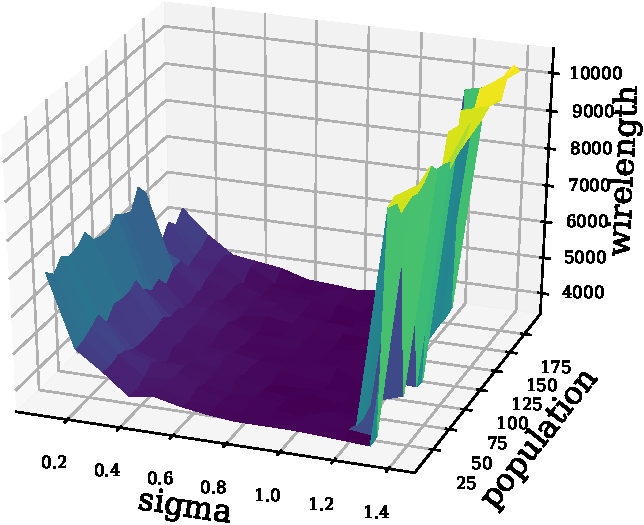
\includegraphics[width=0.6\textwidth]{figure/cma_sensitivity-crop}
	\caption{标题} 
	\label{fig:objective}
\end{figure}

\begin{figure}[h]
	\centering
	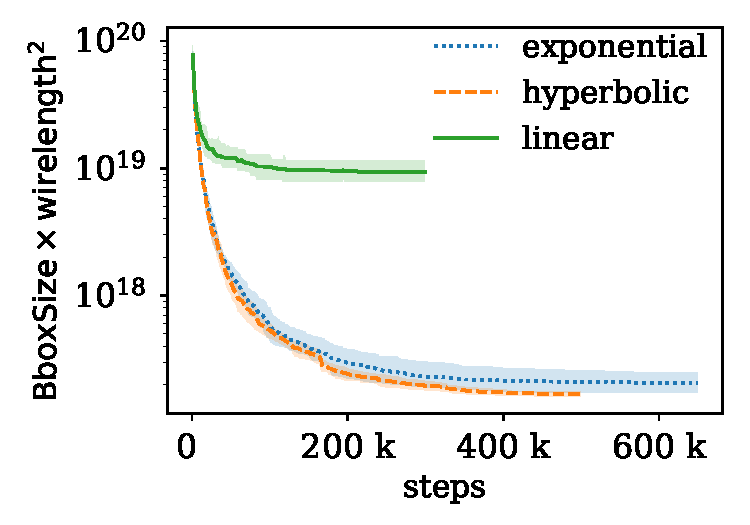
\includegraphics[width=0.6\textwidth]{figure/Annealing-Tuning}
	\caption{标题} 
	\label{fig:objective}
\end{figure}

\begin{figure}[h]
	\centering
	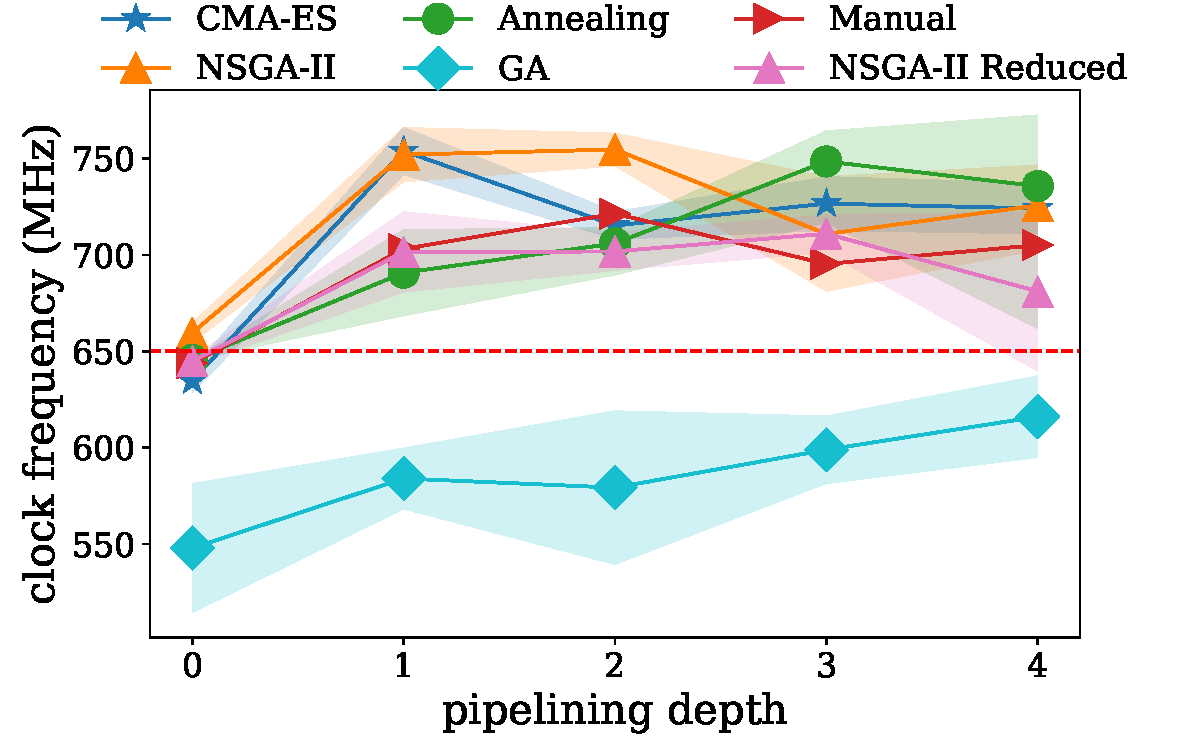
\includegraphics[width=0.8\textwidth]{figure/frequency_depth}
	\caption{标题} 
	\label{fig:objective}
\end{figure}





\section{实验设置以及实验结果}



\subsection{实验设置}


\subsection{性能对比}

\begin{figure}[h]
	\centering
	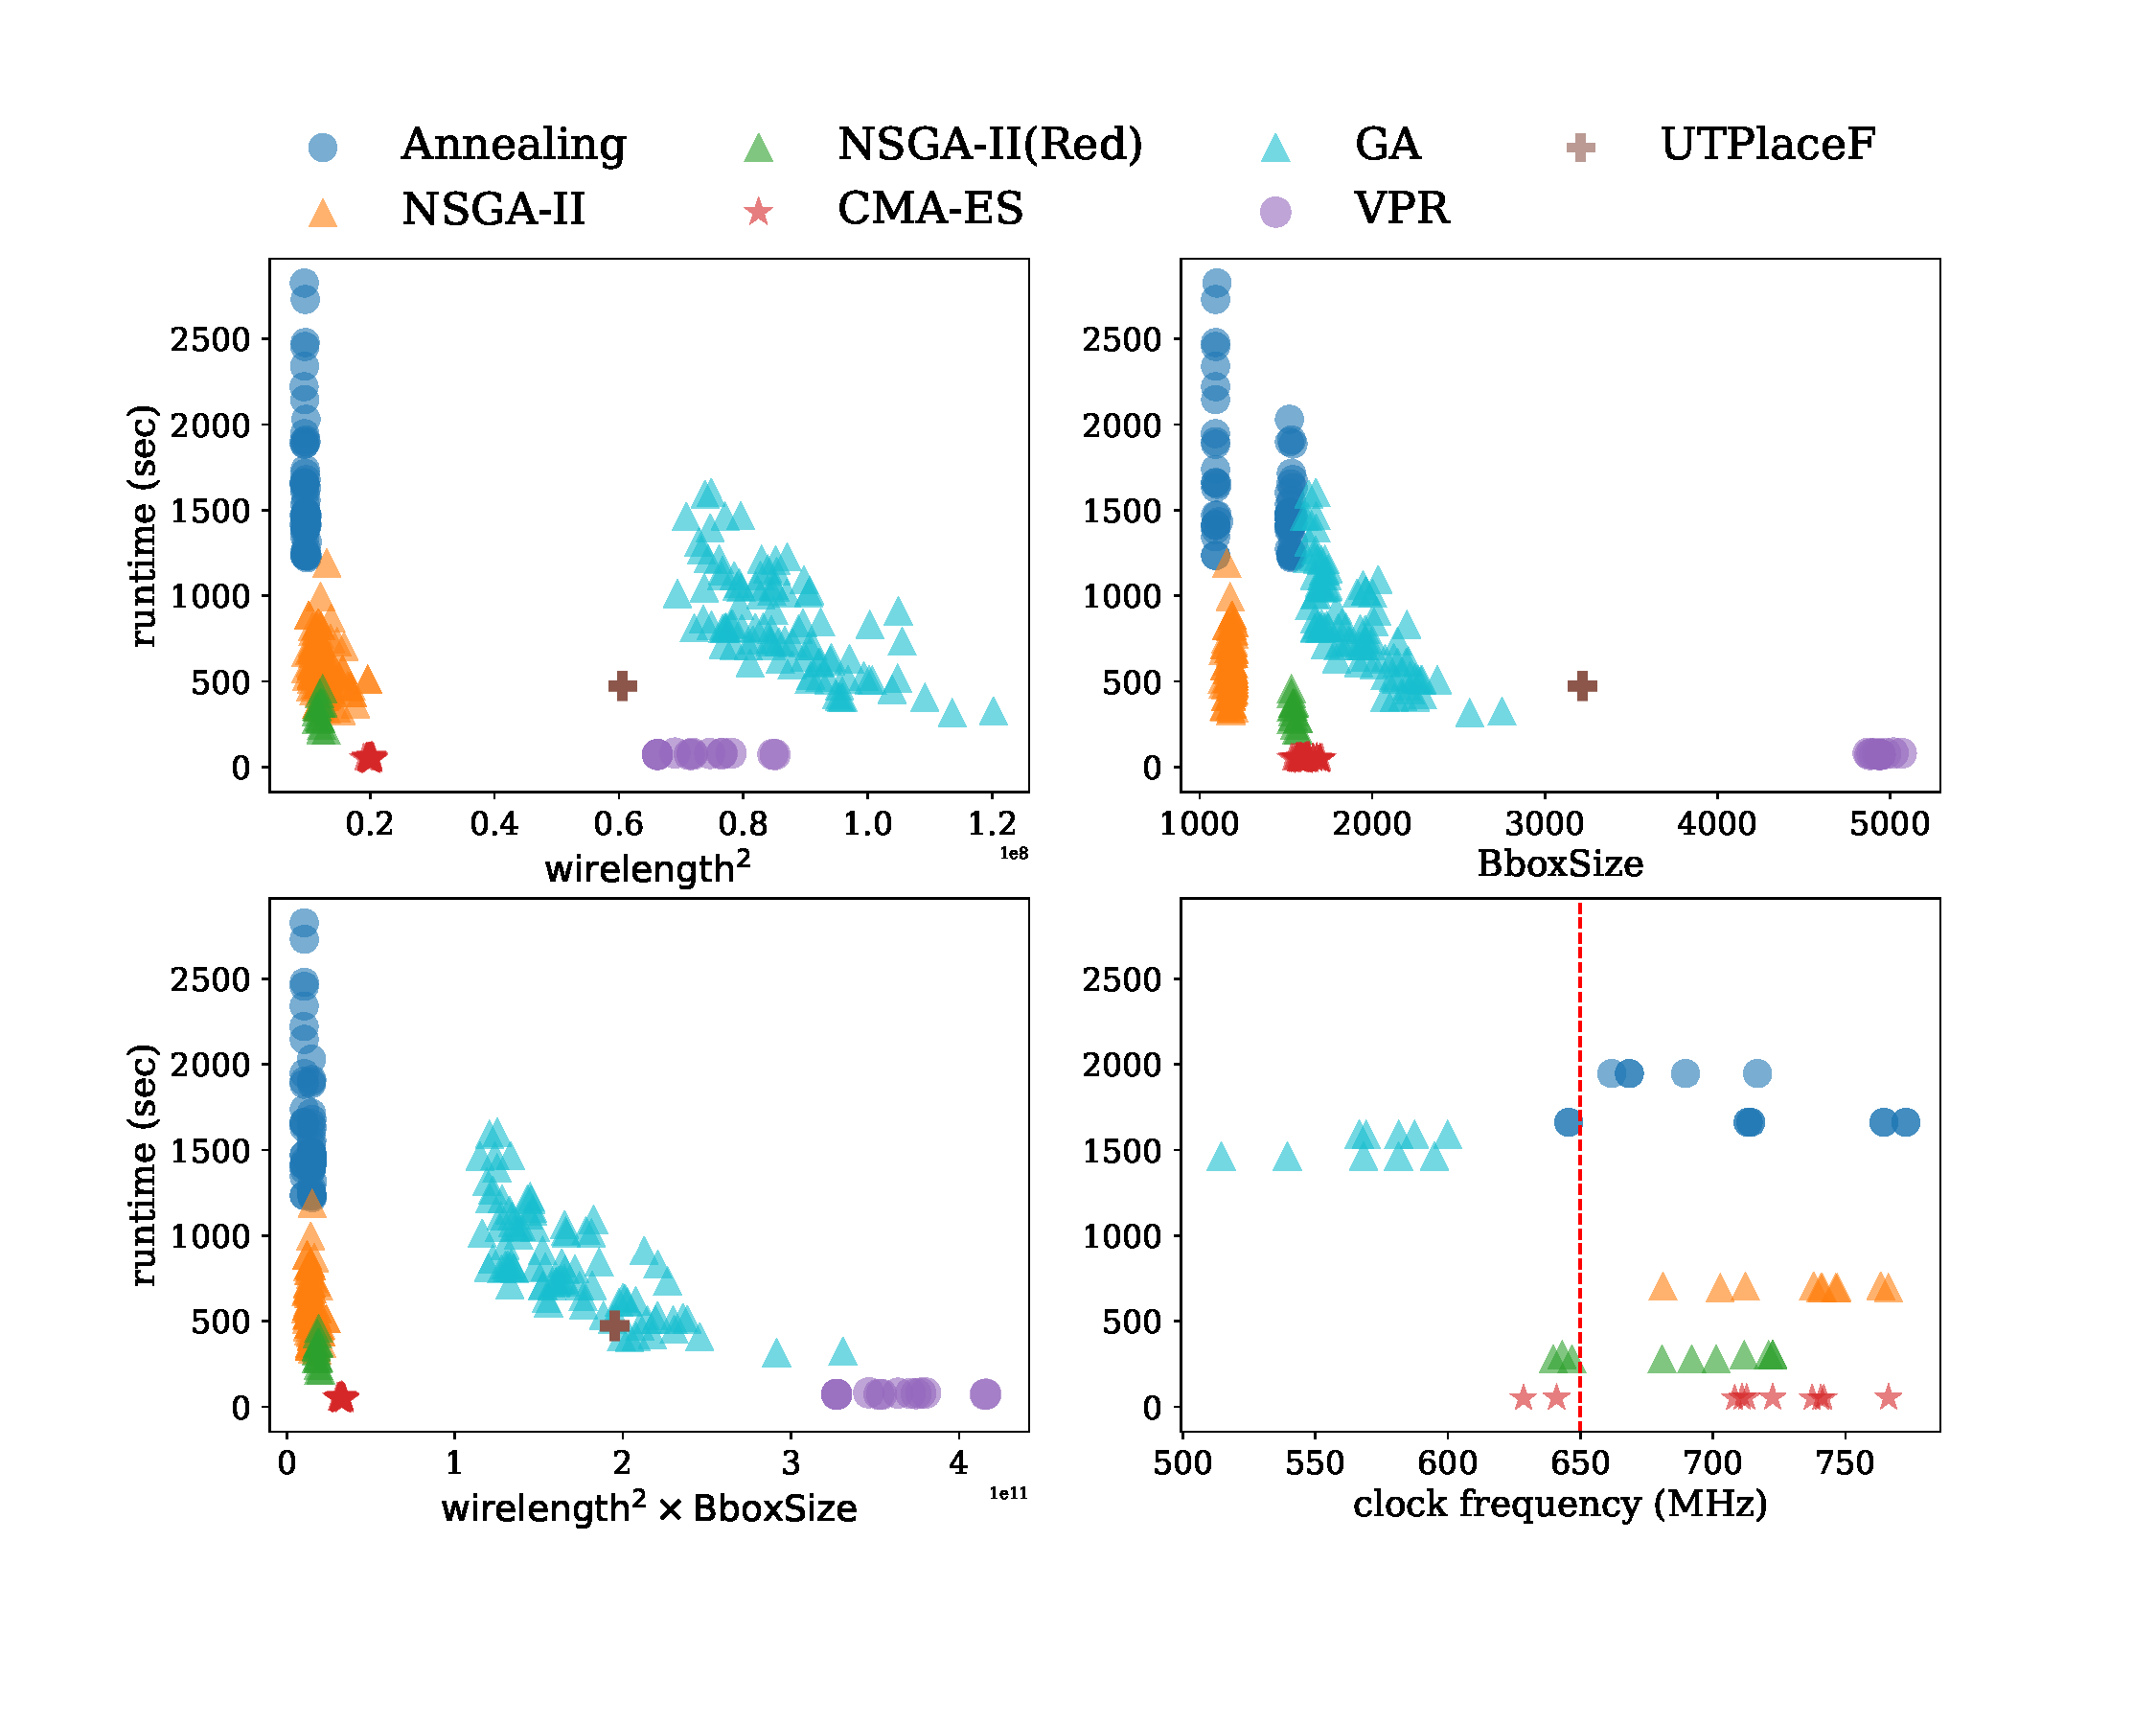
\includegraphics[width=\textwidth]{figure/objective-runtime}
	\caption{标题} 
	\label{fig:objective}
\end{figure}


\begin{figure}[h]
	\centering
	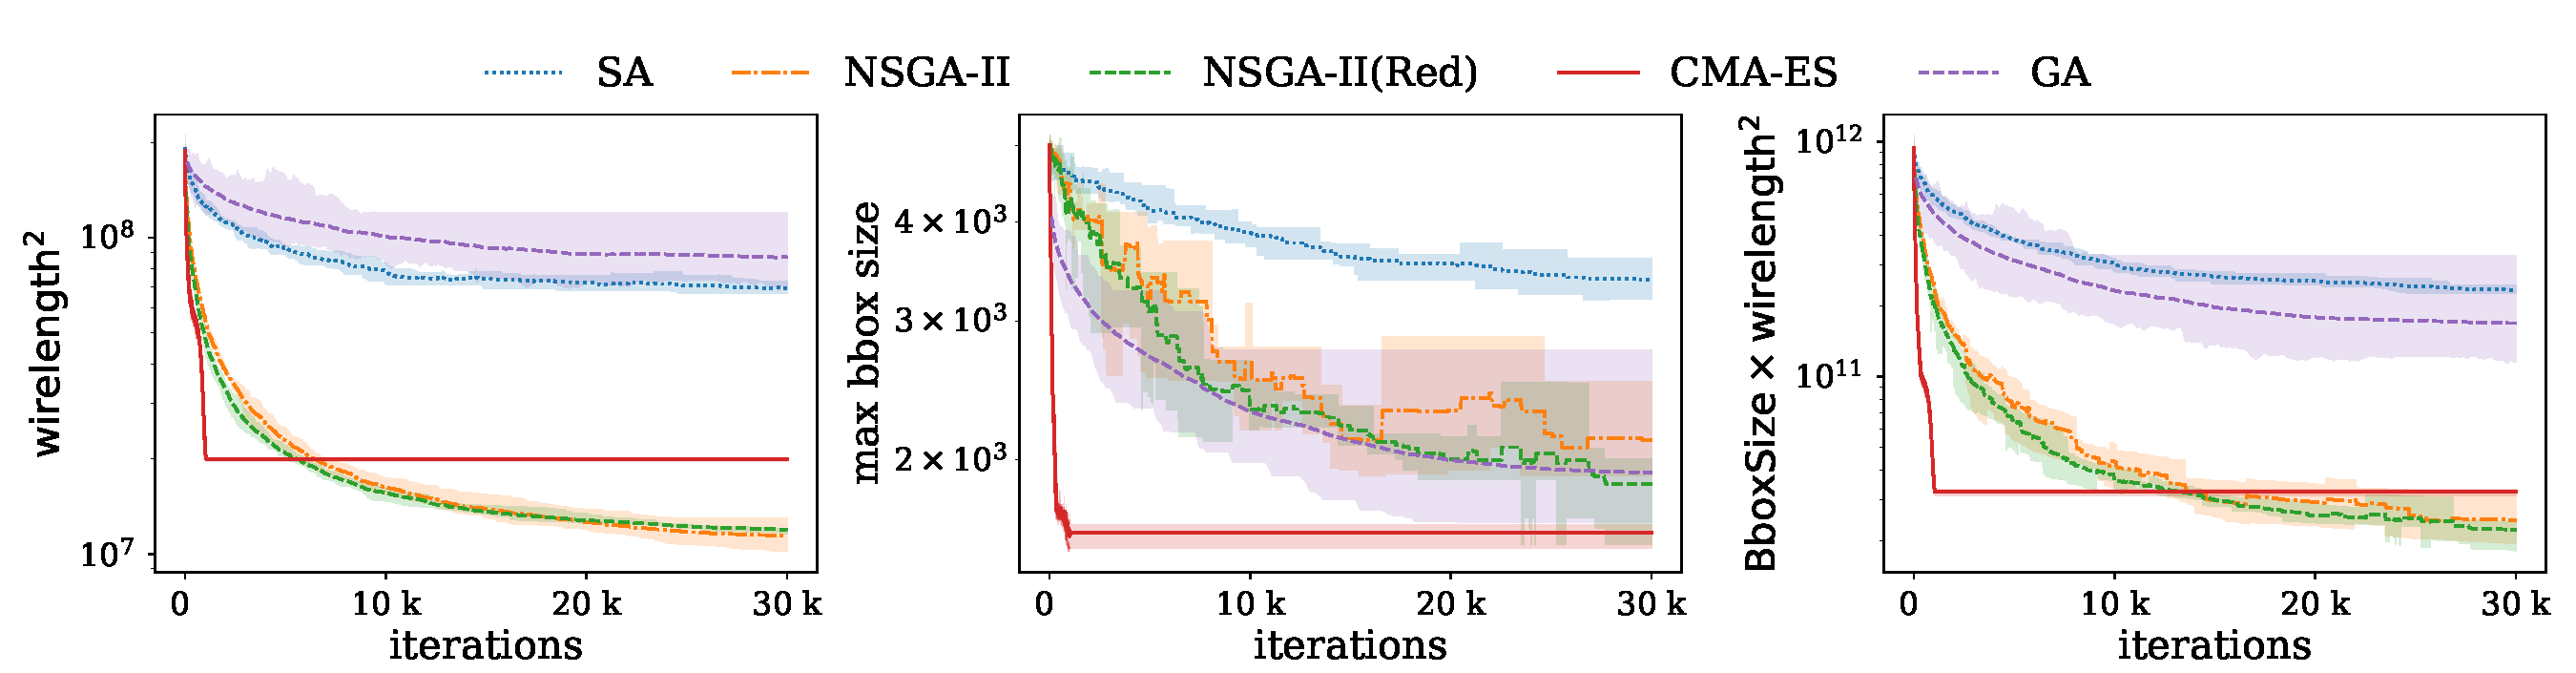
\includegraphics[width=1.1\textwidth]{figure/convergence}
	\caption{标题} 
	\label{fig:converge}
\end{figure}

% table of performance comparison
\begin{table*}[t]
	\caption{Runtime(avg), Wirelength(avg), Max BBox(avg), Pipelining
  Registers(min), and Frequency(avg) for all methods. NSGA-II shows reduced
genotype as well. Speeups and QoR improvements wins by Evolutionary algorithms
also reported in \textcolor{red}{red}$\rightarrow$NSGA-II and \textcolor{olive}{green}$\rightarrow$CMA-ES 
for each competitor algorithm (SA, GA, UTPlaceF, VPR, Manual).}	
	\label{table:comparison}
  \centering
  \begin{adjustbox}{width=1.1\textwidth,center}
  \begin{tabular}{c|c c| c c c c c}
	\toprule
  Method             & NSGA-II    	          & CMA-ES       & SA 					                                                                       & GA 			                                                                  & VPR     	                                                                & UTPlaceF 		                                                                   &  Manual \\
	\midrule
  Runtime (secs)     & 586 (323)		          & 51  		     &1577     (\textcolor{red}{2.7$\times$}, \textcolor{olive}{30.8$\times$})		        & 850 (\textcolor{red}{1.5$\times$}, \textcolor{olive}{16.7$\times$})		      & 76 (\textcolor{red}{0.13$\times$}, \textcolor{olive}{1.5$\times$})		    &  473 (\textcolor{red}{0.8$\times$}, \textcolor{olive}{9.3$\times$})            & 1--2 wks\\
  Wirelength  	     & 3.5K  (3.5K)   		    & 4.4K     		 &3.1K 	   (\textcolor{red}{0.9$\times$}, \textcolor{olive}{0.7$\times$})		          & 9.2K  (\textcolor{red}{2.6$\times$}, \textcolor{olive}{2.1$\times$})    		& 8.5K (\textcolor{red}{2.4$\times$}, \textcolor{olive}{1.9$\times$})   		&  7.8K  (\textcolor{red}{2.2$\times$}, \textcolor{olive}{1.8$\times$})          & 8.1K (\textcolor{red}{2.3$\times$}, \textcolor{olive}{1.8$\times$})  \\
  BBox      	       & 1183  (1543)   		    & 1606     		 &1387	   (\textcolor{red}{1.2$\times$}, \textcolor{olive}{0.9$\times$})		          & 1908  (\textcolor{red}{1.6$\times$}, \textcolor{olive}{1.2$\times$})   		  & 4941	(\textcolor{red}{4.1$\times$}, \textcolor{olive}{3.1$\times$})  		&   3218	(\textcolor{red}{2.7$\times$}, \textcolor{olive}{2.0$\times$})         & 1785 (\textcolor{red}{1.5$\times$}, \textcolor{olive}{1.1$\times$})  \\
  Pipeline Reg.		   & 256K  (273K) 		      & 273K	   		 &273K	   (\textcolor{red}{1.1$\times$}, \textcolor{olive}{1$\times$}) 	 	          & 323K	(\textcolor{red}{1.3$\times$}, \textcolor{olive}{1.2$\times$})   		  & -		                                                                      &   -                                                                            & 306K (\textcolor{red}{1.2$\times$}, \textcolor{olive}{1.1$\times$})   \\
  Frequency	(MHz)	 	 & 733  (688)   & 708 	 &711  (\textcolor{red}{0.97$\times$}, \textcolor{olive}{1.0$\times$})		        & 585 	(\textcolor{red}{0.80$\times$}, \textcolor{olive}{0.83$\times$})	& - 	      	                                                              & - 	                                                                           & 693 (\textcolor{red}{0.95$\times$}, \textcolor{olive}{0.98$\times$}) \\
	\bottomrule
	\end{tabular}
  \vspace{-0.2in}
\end{adjustbox}
\end{table*}



\subsection{收敛情况对比}


\subsection{流水线}


\subsection{布局迁移学习}

\begin{table}[h!]
    \caption{Transfer Learning Performance: VU3P, VU11P as Seed Devices}
    \label{table:port}
    \centering
    \begin{adjustbox}{width=0.8\columnwidth,center}
    \begin{tabular}{c|c c c c c}
      \toprule
  \multirow{2}{*}{Device}     & Design Size 		& Impl.Runtime 		& Frequency 	 & \multicolumn{2}{c}{Placement Runtime}    			\\ \cline{5-6}
                                 & (conv units)		& (mins.)				& (MHz)			 & 	Scratch (s)			& 	Transfer (s)				\\
      \midrule
      \emph{xcvu3p}  			& 123				&	46.4			& 718.9			 & 428.3				& - 							\\
      \emph{xcvu5p}  			& 246				&   56.9				& 677.9	 		 & 396.0				& 55.7 	(\textcolor{red}{7.1$\times$})							\\
      \emph{xcvu7p}  			& 246			    &   55.1				& 670.2	 		 & 345.4				& 44.2 	(\textcolor{red}{7.8$\times$})							\\
      \emph{xcvu9p}  			& 369	   			&   58.4				& 684.9	 		 & 316.5				& 45.5 	(\textcolor{red}{7$\times$})							\\ 
      \midrule
      \emph{xcvu11p} 			& 480	      	    &	65.2          	& 655.3	 		 & 695.9				& -								\\	
      \emph{xcvu13p} 			& 640        	    & 	69.4   			& 653.2	 		 & 704.9				& 58.8	(\textcolor{red}{12$\times$})			\\
      \bottomrule
    \end{tabular}
    \vspace{-0.1in}
    \end{adjustbox}
  \end{table}q  


\subsection{布局结果展示}

\begin{figure}[t]
	\centering
	\subfloat[Unroutable floorplan in raw Vivado with heavy congestion]{
		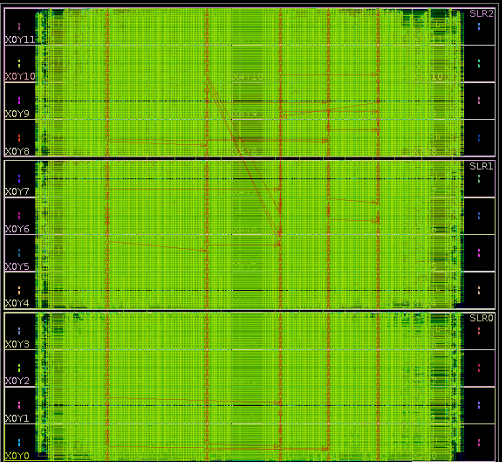
\includegraphics[width=0.3\textwidth, height=0.5\textwidth]{figure/vivado-placed.png}
	}
	\hfill
	\subfloat[Manual constraints in Vivado routes in 5--6 hours.]{
		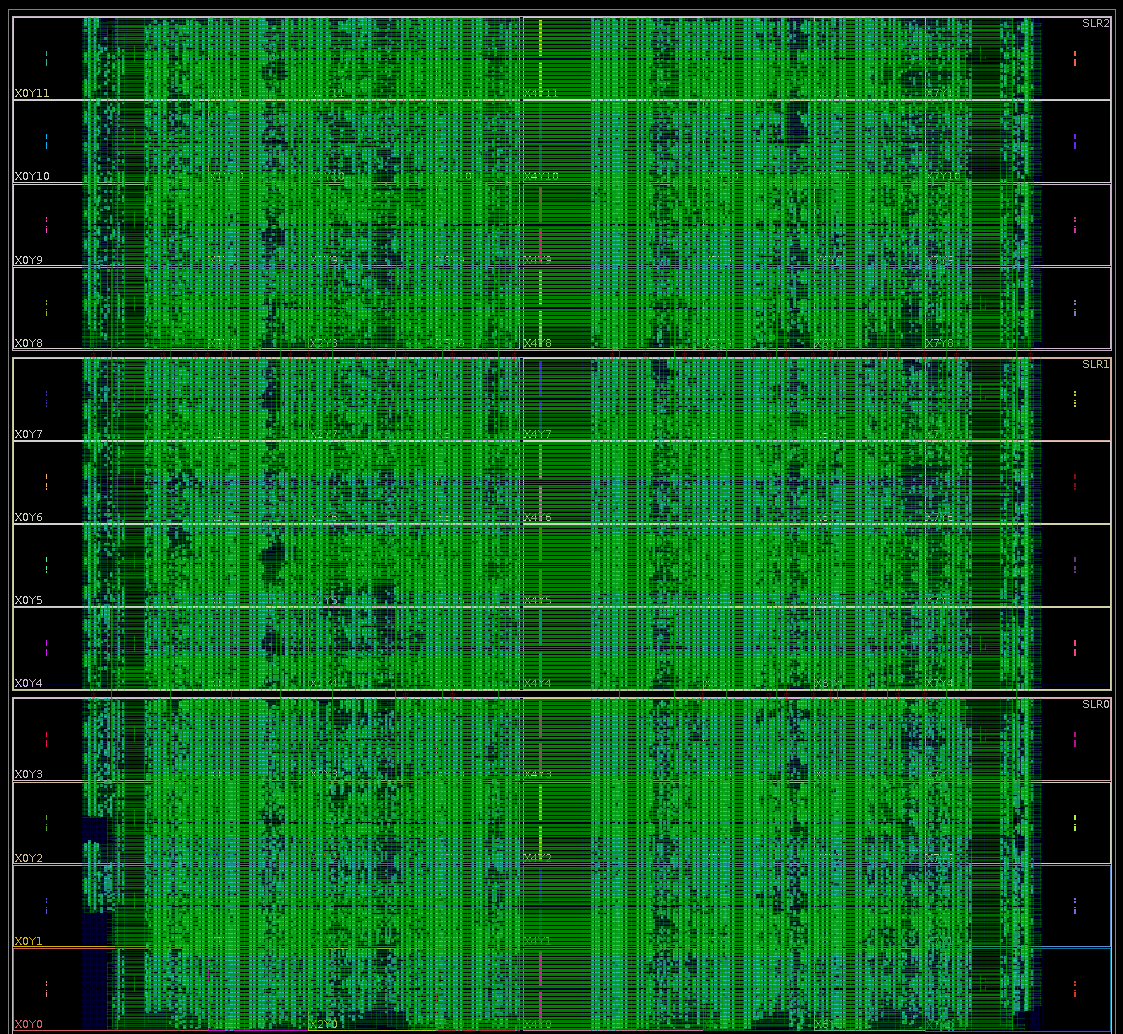
\includegraphics[width=0.3\textwidth, height=0.5\textwidth]{figure/manual-placed.png}
	}
	\hfill
	\subfloat[Automatic mapping with RapidLayout routes in $\approx$1 hour.] {
		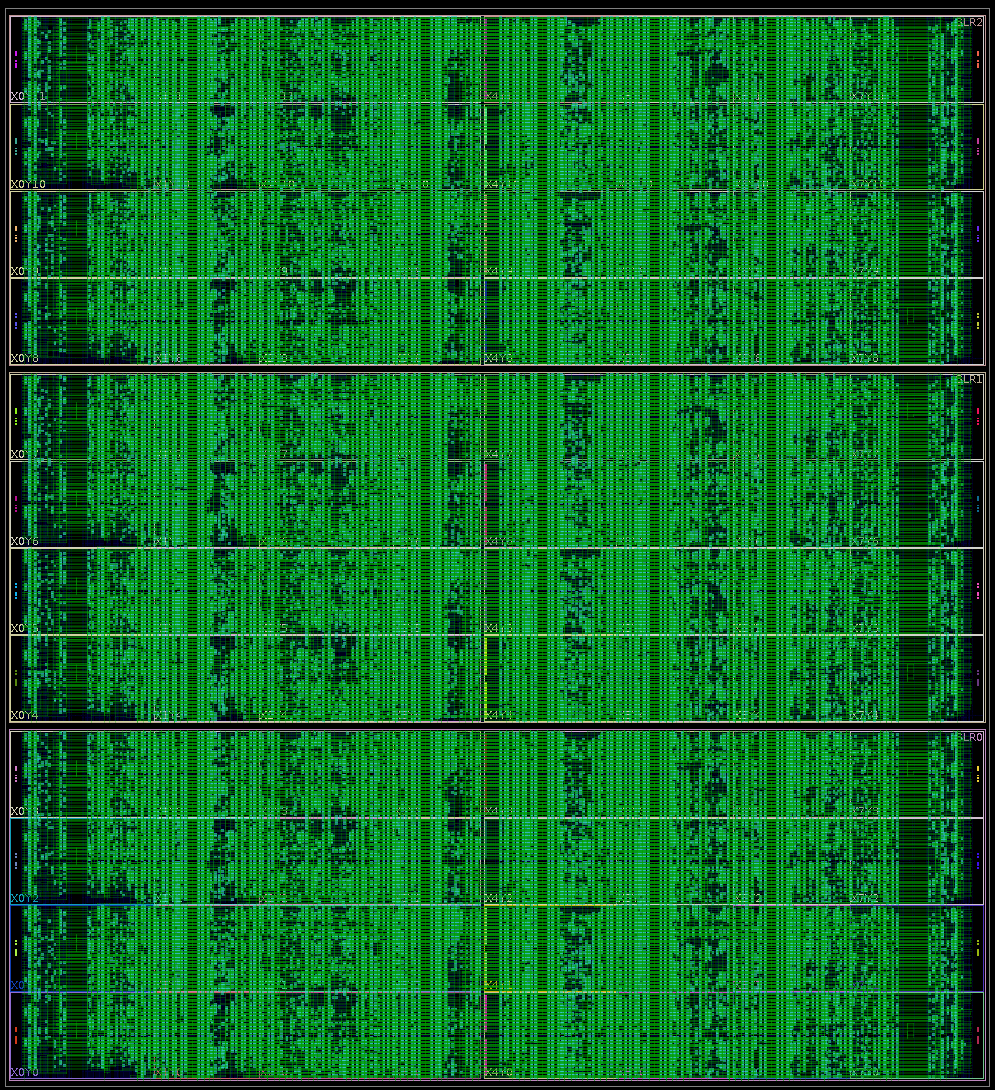
\includegraphics[width=0.3\textwidth, height=0.5\textwidth]{figure/rapidlayout-placed.png}
	}
	\caption{
   Floorplanning scenarios for a neural network accelerator with 480
   convolution blocks mapped to Xilinx UltraScale+ VU11P.}
	\label{fig:overview}
 \vspace{-0.25in}
\end{figure}

\section{本章小结}











































































% \chapter{基于多线索操纵的图像颜色编辑应用}
% 内容概括 \cite{Zuo10}

% \section{多线索操纵图像颜色编辑框架设计}
% 多线索操纵的交互式颜色传递框架集合了基于颜色聚类分割、基于图像修补的边界矫正、梯度保持优化和颜色分布映射等多种手段。……

% \section{多线索操纵图像颜色编辑框架具体实现}
% 多线索操纵图像颜色编辑框架集合了全局图像颜色编辑和局部图像颜色编辑功能。……

% \section{多线索操纵图像颜色编辑实验结果分析}
% 下面将分别给出全局以及局部图像颜色编辑的实验结果对比,并进行分析。……

% \section{本章小结}
% 在本章中,我们提出一种基于多线索操纵的图像颜色编辑方法,介绍图像编辑框架流程。本文采用Mathworks的MATLAB 2010a作为实验平台,结合附带的图像处理工具箱进行算法验证,同时使用MATLAB的GUI设计工具实现了交互式的操作程序,使得实验过程更加直观。实验结果表明,本章所提出的图像编辑框架具有比较强的可操作性和比较理想的处理结果。由于使用 GUI交互操作的方式,因此,用户有了更多的操控自由。


